\subsection*{PCB Ordering \& Assembly Scope}
PCB should be ordered using Gerber files, Pick \& Place, and BOM. Select a 1.6\,mm PCB with standard solder mask and silkscreen colours. The top face should be assembled, with the \textbf{switch} and \textbf{female header pins} left unpopulated for hand-soldering.

\subsection*{Bill of Materials (Selected Items)}
\begin{longtable}{@{}m{2.2cm}m{2cm}m{2cm}m{1.5cm}m{4.5cm}m{2.5cm}@{}}
\toprule
\textbf{Item} & \textbf{Designator} & \textbf{Value/Spec} & \textbf{Qty} & \textbf{Notes / Supplier Ref.} & \textbf{Image}\\
\midrule
Female Header (PM2.54-1*6) & --- & 2.54\,mm socket & 1 & LCSC: \texttt{PM2.54-1*6} & 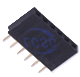
\includegraphics[width=1.6cm]{img/manual/item1.png}\\
WR-PHD 2.54\,mm Socket Header & --- & 2.54\,mm & 1 & DigiKey: \texttt{613006143121} & 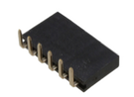
\includegraphics[width=1.8cm]{img/manual/item2.png}\\
ESP32-WROOM-32 & --- & --- & 1 & LCSC: \texttt{ESP32-WROOM-32} & 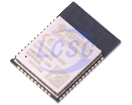
\includegraphics[width=1.8cm]{img/manual/item3.png}\\
Capacitor & C9 & 10\,\textmu F & 1 & LCSC: \texttt{CL10A106KP8NNNC} & 
\includegraphics[width=1.8cm]{img/manual/item4.png}\\
Capacitor & C10 & 100\,nF & 1 & LCSC: \texttt{CC0603KRX7R9BB104} & 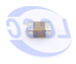
\includegraphics[width=1.8cm]{img/manual/item5.png}\\
Insulated Wire & -- & 16\,guage & 10cm & --- & 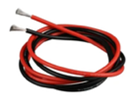
\includegraphics[width=1.8cm]{img/manual/item6.png}\\
E-Switch & SW1/2 & 4\,A max & 1 & DigiKey: \texttt{R4ABLKREDFF0} & 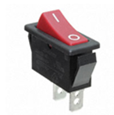
\includegraphics[width=1.4cm]{img/manual/item7.png}\\
\bottomrule
\end{longtable}

\pagebreak
\subsection*{Unboxing \& Visual Inspection Checklist}
\begin{itemize}
  \item[] \checkbox{} Humidity sensing paper indicates no moisture; packaging shows no mechanical damage.
  \item[] \checkbox{} Inspect all soldered joints for bridges or opens; reflow or add solder as needed.
  \item[] \checkbox{} Continuity: verify no shorts between \texttt{3.3V$\rightarrow$GND}, \texttt{5V$\rightarrow$GND}, \texttt{BATT$\rightarrow$GND}.
  \item[] \checkbox{} Join test: mate the JST connector to the PCB-mounted female JST and confirm correct fit.
\end{itemize}

\subsection*{Tools \& Preparation}
\begin{itemize}
  \item Temp-controlled soldering iron (320--360\,$^{\circ}$C or per manufacturer), solder wire, solder wick.
  \item Flux; isopropyl alcohol and swabs; tweezers.
  \item Safety: fume extraction, eye protection, ESD wrist strap (for sensitive parts).
\end{itemize}

\subsection*{Through-Hole Technology (THT) Soldering}
Applicable parts: Female headers (\textit{VLXattachment1 / vlxattachment}), insulated wire, E-switch.
\begin{itemize}
  \item Apply flux to each pin/pad to promote wetting and keep solder confined to the intended land.
  \item Heat the joint (lead + pad), feed solder, then remove solder first and iron second; allow to cool undisturbed.
\end{itemize}

\begin{figure}[h]
  \centering
  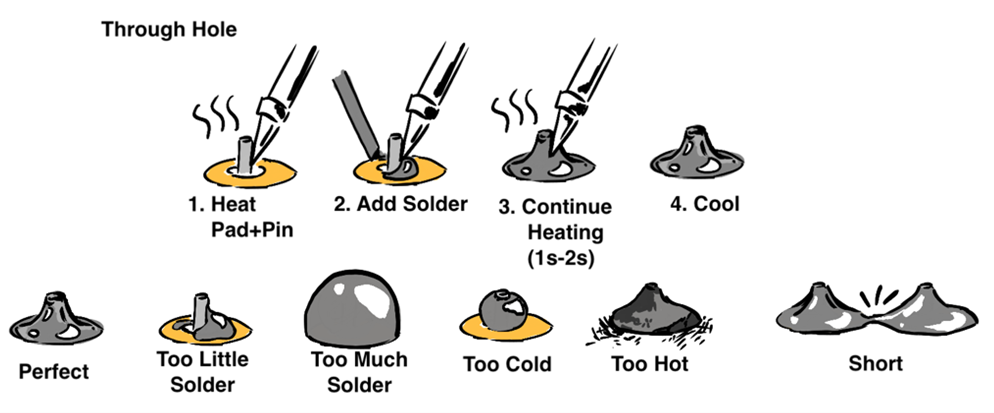
\includegraphics[width=0.5\linewidth]{img/manual/solder1.png}
  % \caption{Through-hole guide}
\end{figure}

\subsection*{Surface Mount Device (SMD) Soldering}
Applicable parts: Capacitors (10\,\textmu F, 100\,nF), ESP32-WROOM module.
\begin{itemize}
  \item Apply flux to pads; hold part with tweezers and tack one pad first while pressing gently to avoid tombstoning/lift.
  \item Align ESP32 module precisely; face antenna outwards (off-board edge) before reflowing all pads.
\end{itemize}


\begin{figure}[h]
  \centering
  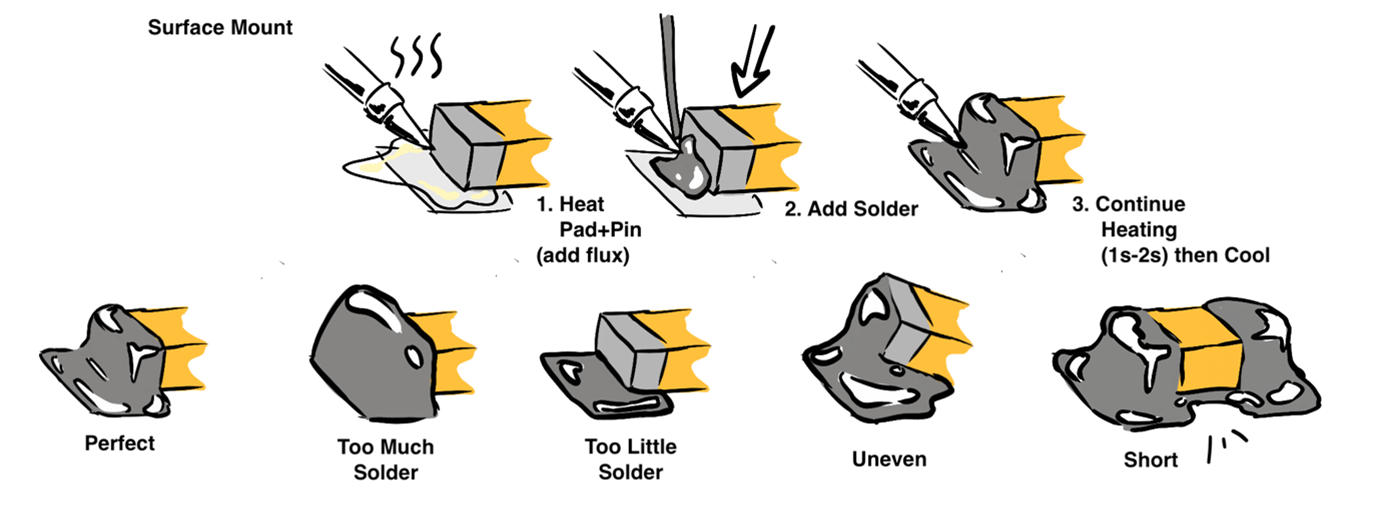
\includegraphics[width=0.5\linewidth]{img/manual/solder2.png}
    % \caption{SMD guide}
\end{figure}

\subsection*{Single-Battery Soldering Steps}
\subsection*{Headers \& Wiring}

\begin{figure}[H]
  \centering
  \begin{subfigure}[b]{0.48\linewidth}
    \centering
    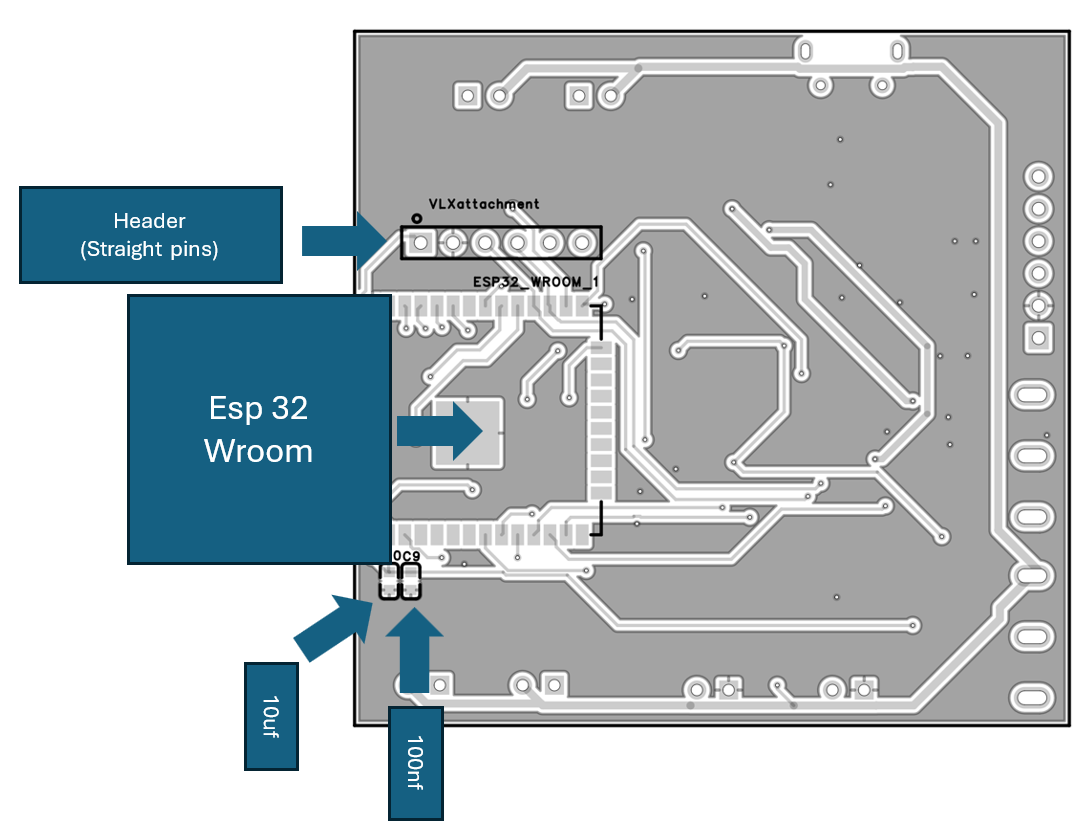
\includegraphics[width=\linewidth]{img/assembly-1.png}
    \caption{Step 1: Back}
  \end{subfigure}
  \hfill
  \begin{subfigure}[b]{0.48\linewidth}
    \centering
    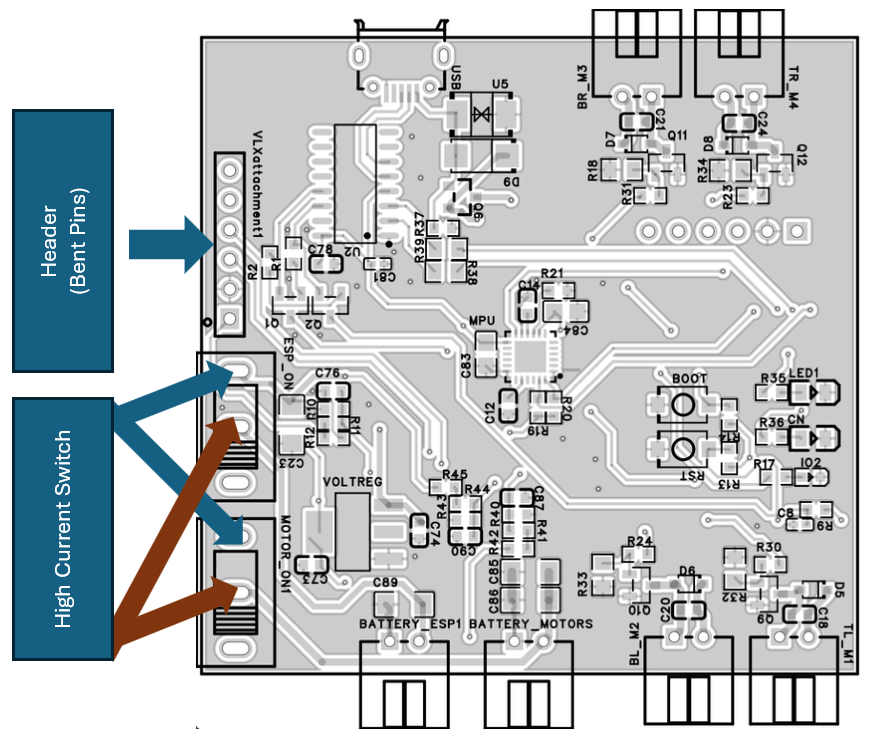
\includegraphics[width=\linewidth]{img/assembly-2.png}
    \caption{Step 2: Front}
  \end{subfigure}
  % \caption{Component Soldering Steps}
\end{figure}

\begin{itemize}
  \item \textbf{WR-PHD 2.54\,mm Socket Header} (\textit{VLXattachment1}): THT. Feed pins through from the board side with header facing outwards; solder.
  \item \textbf{MOTOR\_ON / ESP\_ON} wiring: THT. Use insulated wire and E-switch. Ensure the \emph{ON} configuration bridges as per the diagram.
  \item \textbf{Female Header PM2.54-1*6} (\textit{vlxattachment}): THT. Feed pins through with header facing the user; solder.
\end{itemize}

\subsection*{Modules \& Passives}
\begin{itemize}
  \item \textbf{ESP32\_WROOM\_1} (ESP32-WROOM-32): SMD. Antenna faces outward past board edge; verify pad alignment prior to soldering.
  \item \textbf{C9/C10} (10\,\textmu F/100\,nF): SMD. Ensure no short across capacitor pads after soldering.
\end{itemize}

\subsection*{Rework \& Cleanup}
\begin{itemize}
  \item \textbf{Shorts}: add flux and reflow; if needed, use solder wick to remove excess and retry.
  \item \textbf{Excess/Insufficient Solder}: wick excess or add a small amount, then brief reflow.
  \item \textbf{Flux Residue}: clean with IPA-soaked swabs until pads are clean and matte.
\end{itemize}

\subsection*{Post-Soldering Verification}

\begin{figure}[H]
  \centering
  \begin{subfigure}[b]{0.48\linewidth}
    \centering
    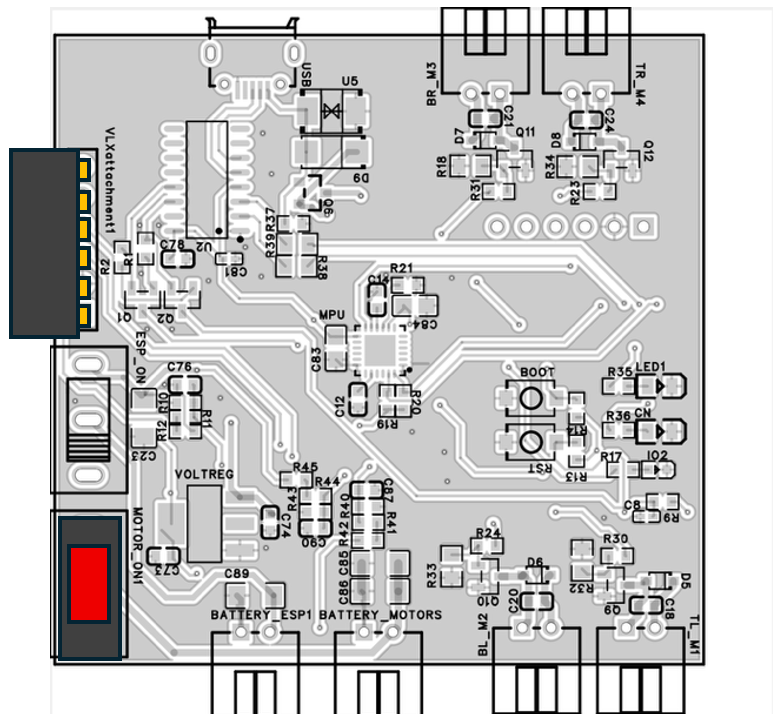
\includegraphics[width=\linewidth]{img/manual/solder5.png}
    \caption{Step 1: Back}
  \end{subfigure}
  \hfill
  \begin{subfigure}[b]{0.48\linewidth}
    \centering
    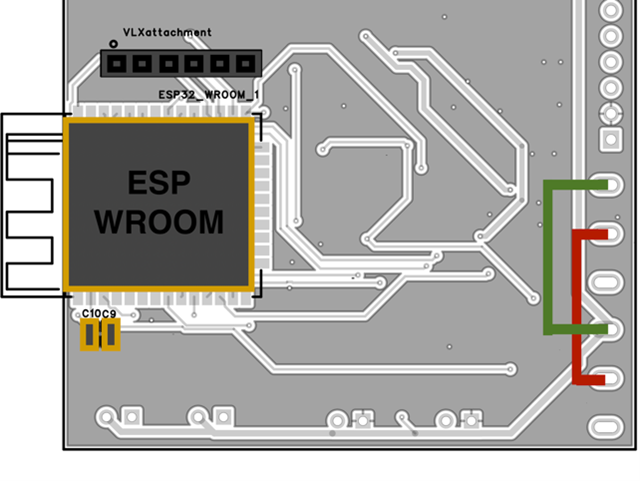
\includegraphics[width=\linewidth]{img/manual/solder6.png}
    \caption{Step 2: Front}
  \end{subfigure}
  % \caption{Soldering Steps}
\end{figure}


\subsection*{Checklist}
\begin{itemize}
  \item[] \checkbox{} Continuity: all ESP32 pins are isolated (no unintended bridges).
  \item[] \checkbox{} Switch continuity and actuation verified (ON/OFF as expected).
  \item[] \checkbox{} C10/C9 terminal isolation confirmed (no shorts).
  \item[] \checkbox{} Visual: all solder joints smooth, shiny, and confined to pad/pin.
  \item[] \checkbox{} Join test: distance sensor module mates correctly in female headers.
\end{itemize}

\subsection*{3D-Printed Frame (PETG)}
The frame is to be printed in PETG. Slice locally with:
\begin{itemize}
  \item Infill: 7\% (gyroid pattern).
  \item Supports: tree supports enabled.
  \item Raft: enabled for plate adhesion.
\end{itemize}

\subsection*{Print QA Checklist}
\begin{itemize}
  \item[] \checkbox{} Layers: consistent adhesion with no gaps.
  \item[] \checkbox{} Edges: no warping present.
  \item[] \checkbox{} Walls: smooth, no bumps or cracks.
  \item[] \checkbox{} Bend test: parts flex slightly and return without splitting (if not, filament may be old/wet).
\end{itemize}

\begin{figure}[H]
  \centering
  \begin{subfigure}[b]{0.48\linewidth}
    \centering
    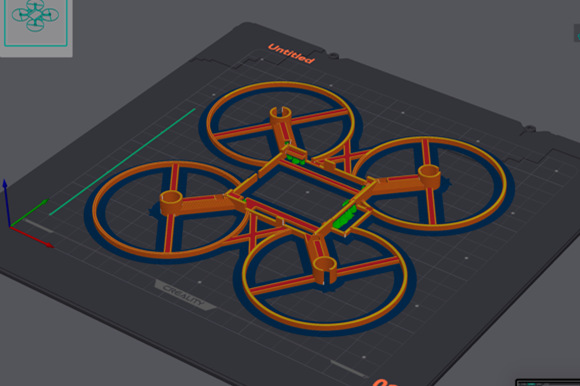
\includegraphics[width=\linewidth]{img/manual/3dp1.png}
    \caption{Main Frame}
  \end{subfigure}
  \hfill
  \begin{subfigure}[b]{0.48\linewidth}
    \centering
    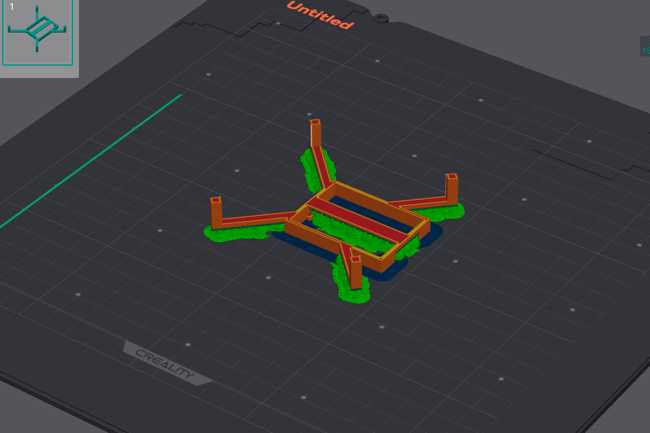
\includegraphics[width=\linewidth]{img/manual/3dp2.png}
    \caption{Camera Mount}
  \end{subfigure}
  \begin{subfigure}[b]{0.48\linewidth}
    \centering
    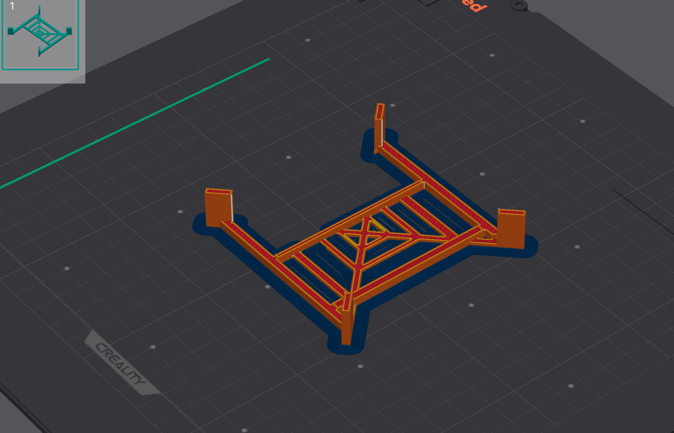
\includegraphics[width=\linewidth]{img/manual/3dp3.png}
    \caption{Battery Cage}
  \end{subfigure}
  \hfill
  \begin{subfigure}[b]{0.48\linewidth}
    \centering
    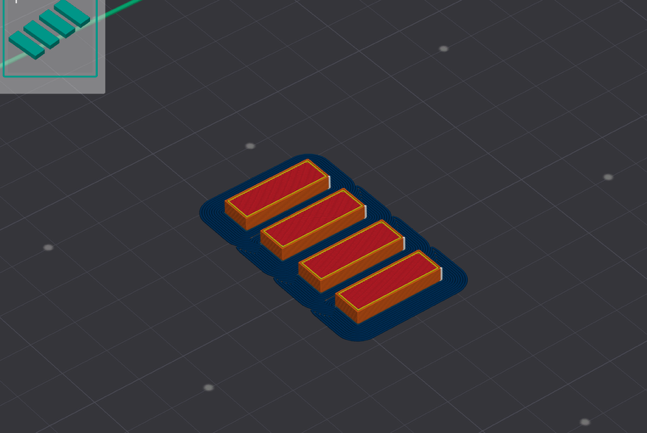
\includegraphics[width=\linewidth]{img/manual/3dp4.png}
    \caption{Feet}
  \end{subfigure}
  % \caption{3D Printing Steps}
\end{figure}


\subsection*{Mechanical Assembly}
\begin{enumerate}
  \item \textbf{Insert PCB}: Flex the main frame slightly at the front; slide the PCB in so frame overhangs rest atop the board. Ensure overhangs do not press on or scrape components.
  \item \textbf{Attach Camera Mount}: Press onto the top of the main frame; align the front with the frame’s front.
  \item \textbf{Attach Battery Cage}: Flip the frame and press the battery cage onto the bottom; maintain correct front orientation.
  \item \textbf{Attach Legs}: Push-fit legs onto the frame.
  \item \textbf{Install Motors}: Push each motor into its hole (friction fit). Ensure CW/ACW motor pairs are mounted diagonally opposite.
  \item \textbf{Install Propellers}: Fit propellers onto matching motor directions (ACW propellers on ACW motors; CW on CW). Propellers should be tight on the shafts.
\end{enumerate}

\begin{figure}[H]
  \centering
  \begin{subfigure}[b]{0.48\linewidth}
    \centering
    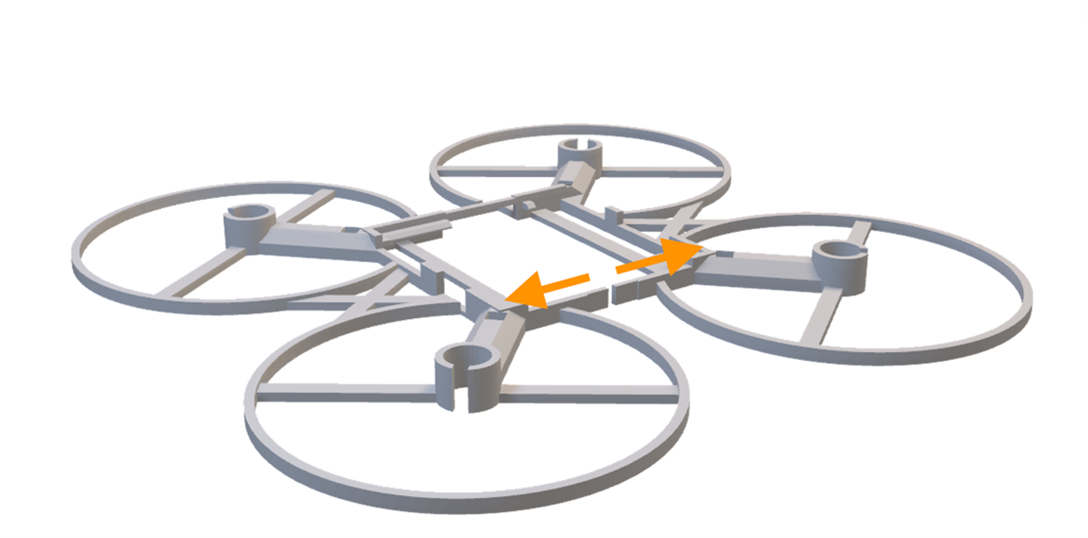
\includegraphics[width=\linewidth]{img/manual/assemb1.png}
    \caption{Main Frame}
  \end{subfigure}
  \hfill
  \begin{subfigure}[b]{0.48\linewidth}
    \centering
    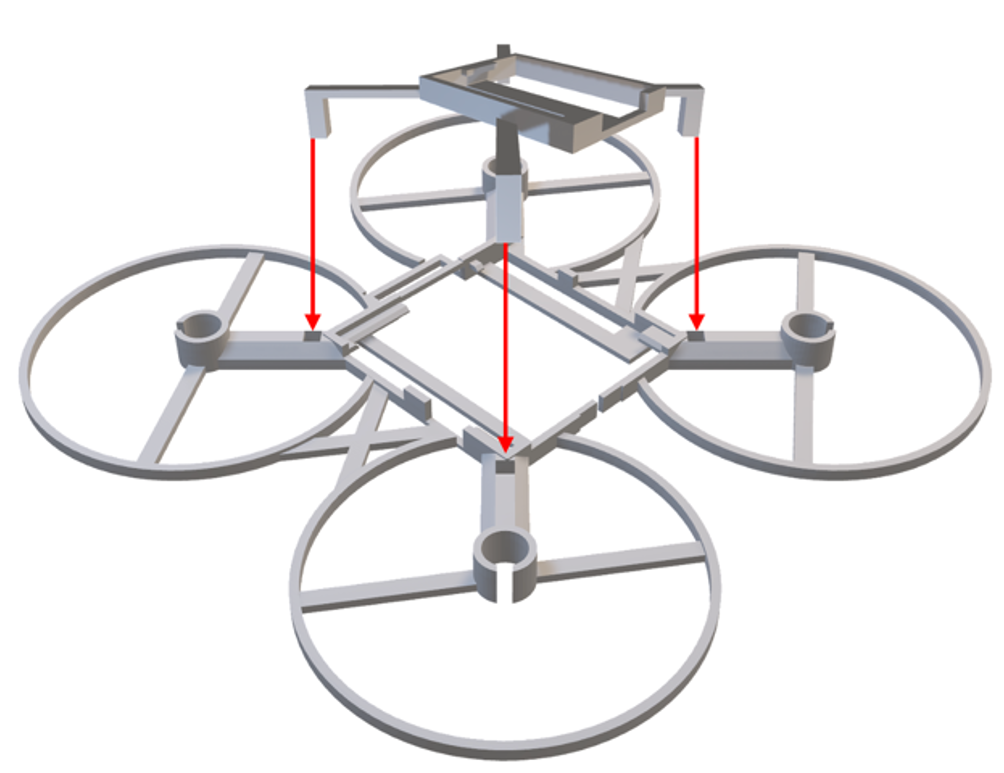
\includegraphics[width=\linewidth]{img/assembly-6.png}
    \caption{Camera Mount}
  \end{subfigure}
  \begin{subfigure}[b]{0.44\linewidth}
    \centering
    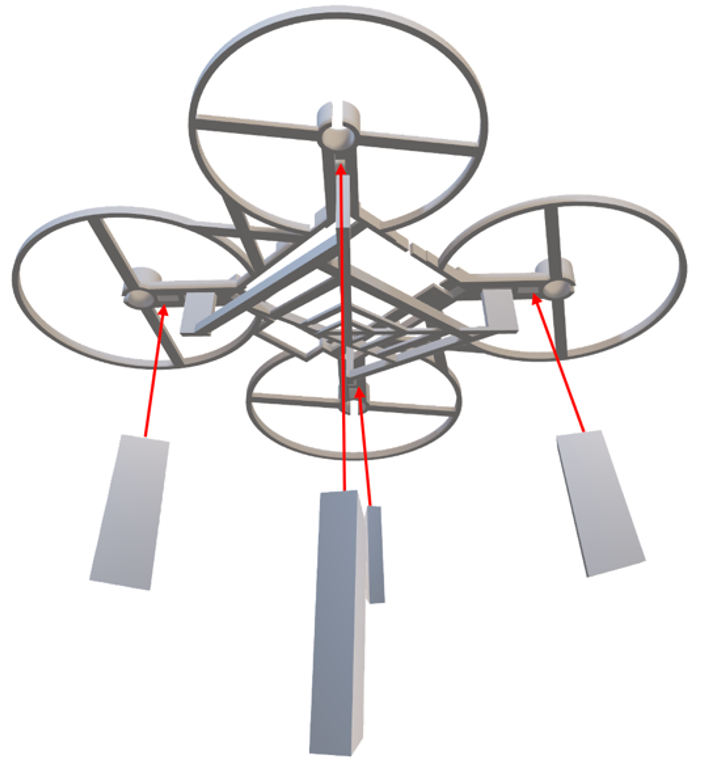
\includegraphics[width=\linewidth]{img/assembly-7.png}
    \caption{Battery Cage}
  \end{subfigure}
  \hfill
  \begin{subfigure}[b]{0.48\linewidth}
    \centering
    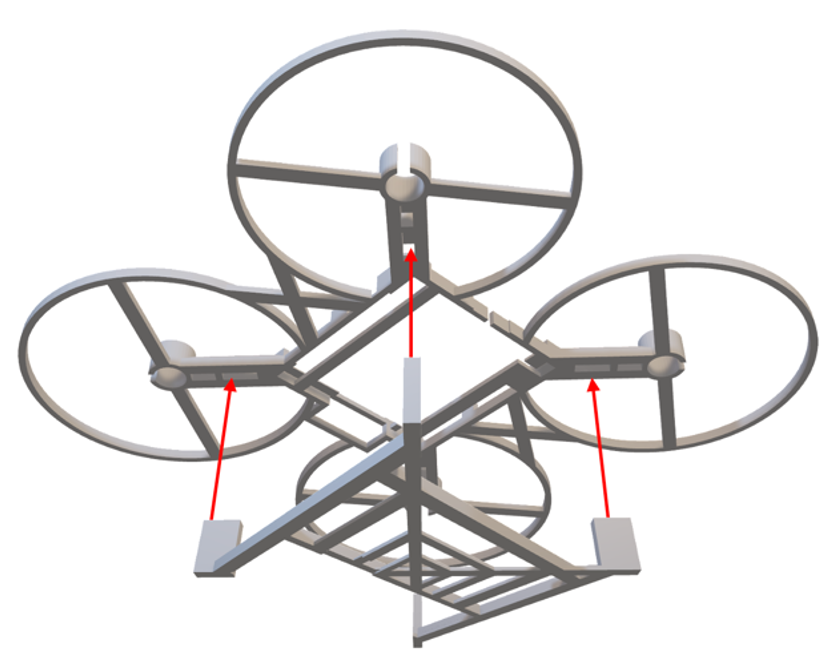
\includegraphics[width=\linewidth]{img/assembly-8.png}
    \caption{Feet}
  \end{subfigure}
  \caption{3D Printing Steps}
\end{figure}

\temp{Add firmware section}